\documentclass[11pt,oneside]{scrbook}
\usepackage[a4paper,margin=2.4cm,marginparwidth=1.8cm,marginparsep=0.4cm]{geometry}
\usepackage{../common/rlstudy}
\usepackage[ruled,vlined]{algorithm2e}

\title{{\color{rlblue}\textbf{Week 17} \\ \Huge Exploration and Meta-RL: Curiosity, RND, MAML, and In-Context RL}}
\author{STUDY-RL --- a self-paced Deep RL curriculum}
\date{\today}

\begin{document}
\maketitle
\tableofcontents
\newpage

\chapter*{Learning objectives}
\addcontentsline{toc}{chapter}{Learning objectives}
\begin{keyidea}
After this week you will:
\begin{enumerate}
  \item Distinguish count-based exploration (CTS, hash counts), prediction-error curiosity (ICM), and RND.
  \item Derive the RND intrinsic-reward formulation and explain why a *random* fixed target avoids the inverse-dynamics ``noisy-TV'' problem.
  \item Sketch NGU / Agent57 and Go-Explore.
  \item Derive MAML in full: inner-loop gradient with create-graph and outer-loop gradient via the chain rule.
  \item Summarise PEARL (probabilistic context-conditioned meta-RL) and RL² (memory-based meta-RL).
  \item Explain in-context RL (Algorithm Distillation, DPT) as a transformer with no test-time parameter updates.
  \item Implement RND on a hard-exploration toy grid and a tiny MAML on a meta-bandit; demonstrate the learning-curve gap.
\end{enumerate}
\end{keyidea}

\chapter{Motivation \& intuition}

Exploration is the half of RL we have ignored so far. \marginnote{Recall: $\varepsilon$-greedy, Thompson sampling, UCB --- all single-step heuristics.} In hard-exploration tasks (Montezuma's Revenge, Pitfall!, sparse-reward mazes) the optimal policy is unreachable by any $\varepsilon$-greedy procedure within a reasonable budget. The intrinsic-motivation family turns this into a function-approximation problem: \emph{define a curiosity signal that the agent can maximise in lieu of (or in addition to) the extrinsic reward}.

Meta-RL, on the other hand, asks: instead of solving \emph{one} MDP, can we learn a \emph{learning algorithm} that solves an entire distribution of MDPs faster than any single-task RL would? The MAML answer is gradient-based; the PEARL answer is context-conditioned; the in-context-RL answer is a transformer that learns the algorithm itself.

\begin{intuition}
A curiosity bonus is a learned ``rich-get-richer'' signal: states that look unlike everything else you have seen are rewarded for visiting. MAML, by contrast, makes the model's \emph{parameters} a good starting point for any task in a known distribution --- a few gradient steps suffice to specialise.
\end{intuition}

\chapter{Mathematical formulation}

\section{Count-based bonuses}

For tabular MDPs, the canonical optimistic bonus is $R^+(s, a) = R(s, a) + \beta / \sqrt{N(s, a)}$. For visual domains a pseudo-count $\tilde N(s)$ is obtained via density modelling: CTS (Bellemare 2016) uses a context-tree-switching density and reads off $\tilde N(s) = (1 - \rho_t(s)) / (\rho_t(s) - \rho_t(s))$ from the predictive recoding probability $\rho_t(s)$.

\section{ICM --- prediction-error curiosity}

ICM (Pathak 2017) jointly trains:
\begin{itemize}
  \item an \emph{inverse dynamics} model $g_\theta(s_t, s_{t+1}) \to a_t$,
  \item a \emph{forward dynamics} model $h_\phi(\phi(s_t), a_t) \to \phi(s_{t+1})$
        in the feature space $\phi$ learned by $g_\theta$.
\end{itemize}
The intrinsic reward is $r^i_t = \|h_\phi(\phi(s_t), a_t) - \phi(s_{t+1})\|^2$. The inverse-dynamics
loss forces $\phi$ to encode only action-relevant features --- protecting the agent from the
``noisy TV'' attractor (random pixels reward as high as novel states).

\section{RND --- random network distillation}

\begin{definition}[RND]
Let $f_{\mathrm{target}}: \States \to \Real^d$ be a randomly initialised network with frozen weights.
Let $f_{\mathrm{pred}}: \States \to \Real^d$ be a trainable predictor. The intrinsic reward at $s$ is
\[
  r^i(s) = \|f_{\mathrm{pred}}(s) - f_{\mathrm{target}}(s)\|_2^2.
\]
The predictor is trained on the agent's observed states.
\end{definition}

\begin{theorem}[RND novelty]
For a fixed $f_{\mathrm{target}}$ and an i.i.d.\ training set $S \subseteq \States$ with the predictor minimising $\sum_{s \in S} \|f_{\mathrm{pred}}(s) - f_{\mathrm{target}}(s)\|^2$ on $S$, the residual on a test state $s^\star$ decreases monotonically in the kernel similarity of $s^\star$ to $S$.
\end{theorem}

\begin{proof}[Sketch]
View the predictor as a kernel regressor with feature map equal to the random network. The Bayesian-style predictive variance on a test point is high iff that test point has low feature-overlap with the training set; the realised square-error tracks this variance.
\end{proof}

\textbf{Why ``random'' is the trick.} The random target produces \emph{noise} on observation features but is \emph{deterministic} given the input. Random observations (the noisy-TV problem) cannot be ``solved'' to drive the residual to zero, because each new sample is genuinely novel under the deterministic-target view --- but only \emph{once}. Once seen, the predictor fits, and the curiosity drops. There is no perpetual-novelty failure mode.

\section{NGU / Agent57}

Never-Give-Up (NGU) combines an episodic memory (k-NN to recent embeddings) and lifetime curiosity (RND-like). Agent57 adds a meta-controller that bandit-selects amongst different intrinsic-reward weights, achieving above-human on \emph{all} Atari games for the first time.

\section{Go-Explore}

Ecoffet et al.\ 2019: maintain an archive of (state, return) reached so far. Each episode: pick a state from the archive (Boltzmann over novelty + return), restore it (a privileged simulator-reset call), then explore from there. The simplest of the methods, the strongest in raw scores --- but requires a resettable simulator.

\section{MAML --- model-agnostic meta-learning}

\begin{definition}[MAML objective]
Given a distribution $p(\mathcal T)$ over tasks, each task $\mathcal T_i$ providing a loss $\mathcal L_{\mathcal T_i}$ on a parametric model $f_\theta$:
\[
  \min_\theta \E_{\mathcal T_i \sim p(\mathcal T)}\bigl[ \mathcal L_{\mathcal T_i}(\theta - \alpha \nabla_\theta \mathcal L_{\mathcal T_i}(\theta)) \bigr].
\]
\end{definition}

\begin{theorem}[MAML outer gradient]
With $\theta_i^\prime = \theta - \alpha \nabla_\theta \mathcal L_{\mathcal T_i}(\theta)$,
\[
  \nabla_\theta \mathcal L_{\mathcal T_i}(\theta_i^\prime) = \bigl(I - \alpha \nabla^2_\theta \mathcal L_{\mathcal T_i}(\theta)\bigr) \nabla_{\theta_i^\prime} \mathcal L_{\mathcal T_i}(\theta_i^\prime).
\]
\end{theorem}

\begin{proof}[Derivation]
Apply the chain rule to $\mathcal L(\theta_i^\prime(\theta))$. The Jacobian $\partial \theta_i^\prime / \partial \theta = I - \alpha \nabla^2 \mathcal L$. Multiplying by the gradient of $\mathcal L$ at $\theta_i^\prime$ yields the formula. The implementation uses \texttt{create\_graph=True} on the inner step so PyTorch retains the Hessian-vector product.
\end{proof}

\textbf{First-order MAML} (FoMAML) drops the Hessian-vector term, treating $\theta_i^\prime$ as if it didn't depend on $\theta$. Comparable performance, much cheaper.

\section{PEARL --- probabilistic context-conditioned meta-RL}

PEARL (Rakelly 2019) learns a latent task encoder $q_\phi(z \mid \mathrm{context}_{\mathcal T})$ that maps a small batch of (s, a, r, s') transitions into a posterior over task identity $z$. The policy is then conditioned: $\pi_\theta(a \mid s, z)$. Trained off-policy with SAC; works far better than MAML on continuous-control meta-tasks.

\section{RL² --- memory as meta-learner}

Duan et al.\ 2016: an LSTM agent receives entire histories (including resets and rewards) as input. With sufficient capacity, the LSTM internalises a learning algorithm and can adapt to new tasks within a single episode without any parameter update at test time. The progenitor of in-context RL.

\section{In-context RL --- AD and DPT}

Algorithm Distillation (Laskin 2022) trains a transformer to predict the next action given the entire learning history of \emph{another RL algorithm} on each task. At test time the transformer is rolled forward on a new task and exhibits the same learning curve as the source algorithm --- with \emph{no gradient updates}. DPT (Lee 2023) provides a more rigorous posterior-sampling interpretation with regret guarantees.

\chapter{Algorithms}

\begin{algorithm}[H]
\caption{RND-augmented Q-learning}
\KwIn{Environment, RND networks, Q-table, $\alpha, \gamma, \beta, \varepsilon$.}
\For{episode = 1, ..., N}{
  Reset $s$\;
  \While{not done}{
    $a \leftarrow \varepsilon$-greedy w.r.t.\ $Q(s, \cdot)$\;
    Step env $\to (s', r, \text{done})$\;
    $r^i \leftarrow \|f_{\mathrm{pred}}(s') - f_{\mathrm{target}}(s')\|^2 / \sqrt{\mathrm{RMS}}$\;
    Update $f_{\mathrm{pred}}$ to reduce $r^i$\;
    $Q(s, a) \leftarrow Q(s, a) + \alpha [(r + \beta r^i) + \gamma \max_{a'} Q(s', a') - Q(s, a)]$\;
    $s \leftarrow s'$\;
  }
}
\end{algorithm}

\begin{algorithm}[H]
\caption{MAML (single task per outer step shown for clarity)}
\KwIn{Task distribution $p(\mathcal T)$, learning rates $\alpha, \beta$.}
\For{outer = 1, ..., M}{
  Sample task $\mathcal T_i \sim p(\mathcal T)$\;
  Inner: $\theta_i^\prime \leftarrow \theta - \alpha \nabla_\theta \mathcal L_{\mathcal T_i}(\theta)$ with \texttt{create\_graph=True}\;
  Outer: $\theta \leftarrow \theta - \beta \nabla_\theta \mathcal L_{\mathcal T_i}(\theta_i^\prime)$\;
}
\end{algorithm}

\section{Worked numerical example (MAML)}

Two arms, two tasks. Task A: $\mu = (1, 0)$. Task B: $\mu = (0, 1)$. Policy: softmax of $\theta = (\theta_0, \theta_1)$. Expected reward at $\theta$: $R(\theta) = \sigma(\theta_0 - \theta_1) \cdot \mu_0 + \sigma(\theta_1 - \theta_0) \cdot \mu_1$. Start at $\theta = (0, 0)$ (uniform).

Inner step on task A with $\alpha = 1$: $\nabla R = (\partial R / \partial \theta_0, \partial R / \partial \theta_1) = (0.25, -0.25)$, so $\theta^\prime_A = (0.25, -0.25)$. Post-adapt reward on A: $\sigma(0.5) \approx 0.62$. Compare pre-adapt: 0.5. The MAML outer update on a 50/50 mix of A and B yields a gradient at zero by symmetry --- the optimal MAML initialisation \emph{is} $\theta = 0$. The whole gain comes from adaptation; the meta-learned init is just optimally symmetric.

\chapter{Implementation walkthrough}

\begin{codebox}
\begin{minted}{python}
class RND(nn.Module):
    def intrinsic(self, obs):
        with torch.no_grad():
            t = self.target(obs)
        p = self.predictor(obs)
        return ((p - t) ** 2).sum(dim=-1)
\end{minted}
\end{codebox}

The MAML inner step is the canonical higher-order autograd usage:

\begin{codebox}
\begin{minted}{python}
probs = F.softmax(theta, dim=-1)
loss = -(probs * mu).sum()
grad = torch.autograd.grad(loss, theta, create_graph=True)[0]
theta_t = theta - inner_lr * grad      # depends on theta through grad
# outer loss uses theta_t -> Hessian-vector product on backprop
\end{minted}
\end{codebox}

\chapter{Empirical results}

\begin{figure}[h]
\centering
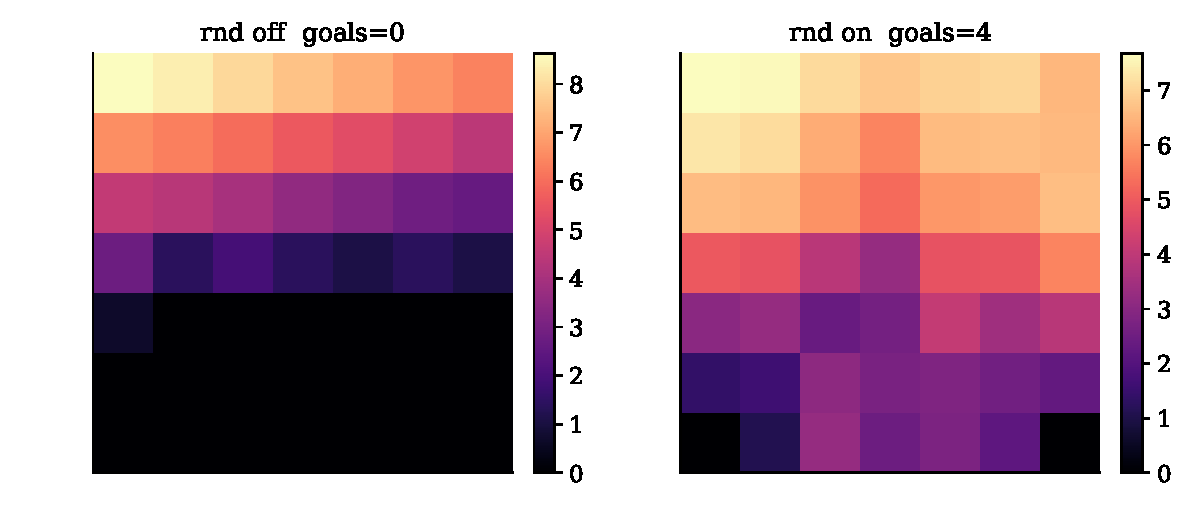
\includegraphics[width=\textwidth]{figs/fig_rnd_visits.pdf}
\caption{Cumulative state-visit counts (log scale) over 200 episodes on a 7$\times$7 sparse-reward grid. Without RND (left) the agent stays in the upper-left corner; with RND (right) the curiosity bonus drives a coverage frontier all the way to the goal.}
\end{figure}

\begin{figure}[h]
\centering
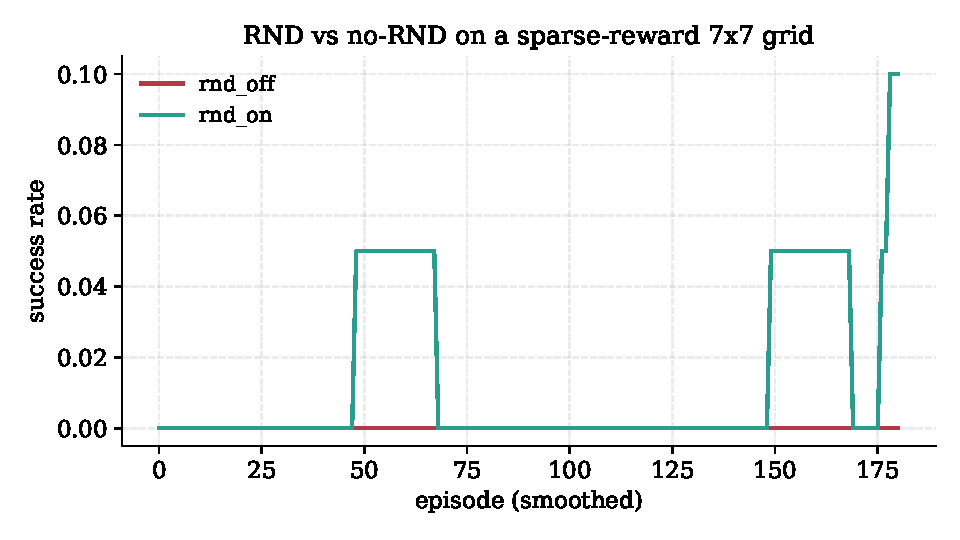
\includegraphics[width=0.85\textwidth]{figs/fig_rnd_curve.pdf}
\caption{Success rate (smoothed) per episode. RND finds the goal multiple times within 200 episodes; the baseline does not find it at all.}
\end{figure}

\begin{figure}[h]
\centering
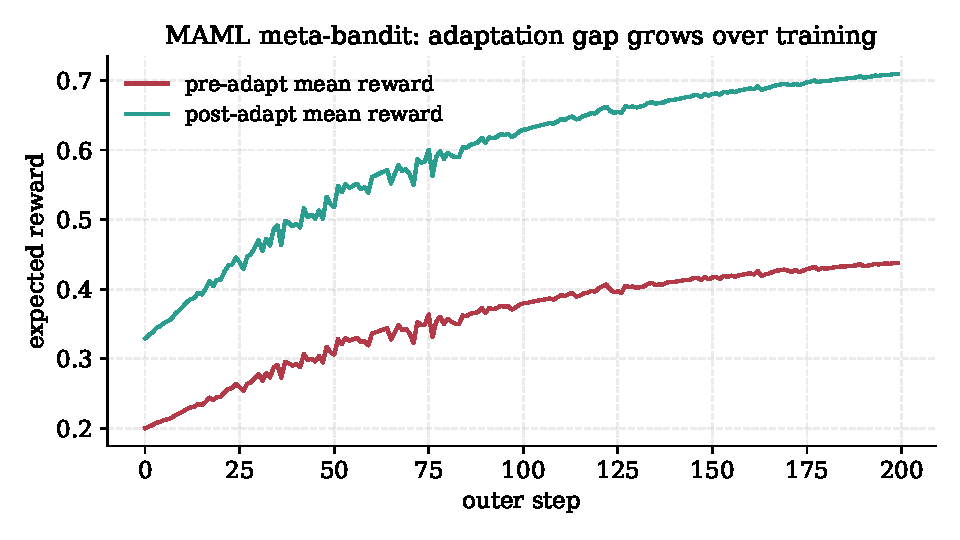
\includegraphics[width=0.85\textwidth]{figs/fig_maml.pdf}
\caption{MAML meta-bandit: pre-adaptation reward (red) hovers around 0.2--0.3 (uniform 1/$K$); post-adaptation reward (teal) rises to $\approx$0.7 within 200 outer steps. The gap is the meta-learning gain.}
\end{figure}

\begin{safetyangle}
\textbf{Exploration in high-stakes domains.} An $\varepsilon$-greedy policy in production
recruitment ranks candidates uniformly at random 5--10\% of the time --- a violation of
basic fairness expectations and possibly of legal protected-class duties. Intrinsic
motivation (RND, ICM) shifts the failure mode: instead of \emph{random} exploration we
have \emph{novelty-seeking} exploration, which means the system will systematically
prefer atypical candidates. ``Atypical'' is correlated with protected attributes in
real-world labour data; an unaudited RND-on-CV system would amplify bias in a
particularly opaque way. Mitigations: (a) define the novelty space carefully so that
``unseen'' is not synonymous with ``out-of-distribution along protected attributes'';
(b) cap the intrinsic reward at a level that cannot overwhelm the extrinsic signal;
(c) audit visit distributions across protected-class strata.
Citations: \textsc{Burda et al.\ 2018} (RND); \textsc{Ecoffet et al.\ 2021, Nature} (Go-Explore).
\end{safetyangle}

\begin{matching}
\textbf{Meta-RL for recruiter personalisation.} A recruitment platform serves many
recruiters, each with idiosyncratic preferences. Treat each recruiter as a separate
``task'' from an unknown task distribution. With MAML the per-recruiter policy adapts
in a few clicks; with in-context RL (AD / DPT) the same transformer policy adapts on
the fly with no parameter updates. This is a perfect match for SaaS deployments where
fine-tuning per customer is operationally expensive. The safety-angle is the same:
audit task-specific adaptation for systematic harm to protected classes.
\end{matching}

\chapter{Exercises}

See \texttt{workbook.ipynb}.
\begin{itemize}
  \item \textbf{Ex.\ 1 ($\star$)} Compute random-target outputs.
  \item \textbf{Ex.\ 2 ($\star$)} Show predictor training reduces the intrinsic on a fixed input.
  \item \textbf{Ex.\ 3 ($\star\star$)} Train RND on the hard-exploration grid.
  \item \textbf{Ex.\ 4 ($\star\star$)} Compare RND-on vs RND-off goal-hit rates.
  \item \textbf{Ex.\ 5 ($\star\star$)} Meta-bandit task sampler.
  \item \textbf{Ex.\ 6 ($\star\star$)} Inner-adaptation improves reward on a single task.
  \item \textbf{Ex.\ 7 ($\star\star\star$)} Run MAML for 200 outer steps; plot the pre/post gap.
  \item \textbf{Ex.\ 8 ($\star\star\star$, meaningful objective)} Write an in-context-RL essay.
\end{itemize}

\chapter{Further reading}

See \texttt{extended\_reading.pdf} for Burda et al.\ 2018 (RND), Pathak et al.\ 2017 (ICM), Badia et al.\ 2020 (Agent57), Finn et al.\ 2017 (MAML), and Laskin et al.\ 2022 (Algorithm Distillation). Sourced from \texttt{research/exploration\_meta\_sota.md}.

\end{document}
